\documentclass{standalone}
\usepackage{mintikz}

\tikzset{oplus/.style={path picture={% 
            \draw[black]
             (path picture bounding box.south west) --
             (path picture bounding box.north east) 
             (path picture bounding box.north west) --
             (path picture bounding box.south east);
            }},
        process/.style={draw, diamond, rounded corners,
            fill=Orchid!30, scale=0.5},
        inout/.style={draw, rectangle, rounded corners,
            fill=cornflowerblue!20},
        inter/.style={draw, ellipse, fill=orange!40,
            scale=0.5},
        add/.style={draw, circle, oplus},
} 

\begin{document}
\begin{tikzpicture}[node distance=1cm, on grid, >=stealth']
    % Do inouts
    \node[inout]
        (data) {Donn\'ees};
    \node[inout, right=of data, xshift=2cm]
        (biascor) {BiasCor};
    \node[inout, below=of data, xshift=1.5cm,
         anchor=north, fill=white,
         minimum width=6cm, minimum height=5.5cm]
        (boxproc) {};
    \node[inout, minimum width=6cm, anchor=north, fill=Orchid!30]
        (bbc5D) at (boxproc.north) {\texttt{BBC5D} + \texttt{SALT2mu}};
    \node[inner sep=0] (chainleft) at (data|-bbc5D.south) {};
    \node[inner sep=0] (chainleftop) at (data|-bbc5D.north) {};
    \node[inner sep=0] (chainright) at (biascor|-bbc5D.south) {};
    \node[inner sep=0] (chainrightop) at (biascor|-bbc5D.north) {};
    \node[below=of chainright]
        (mcube) {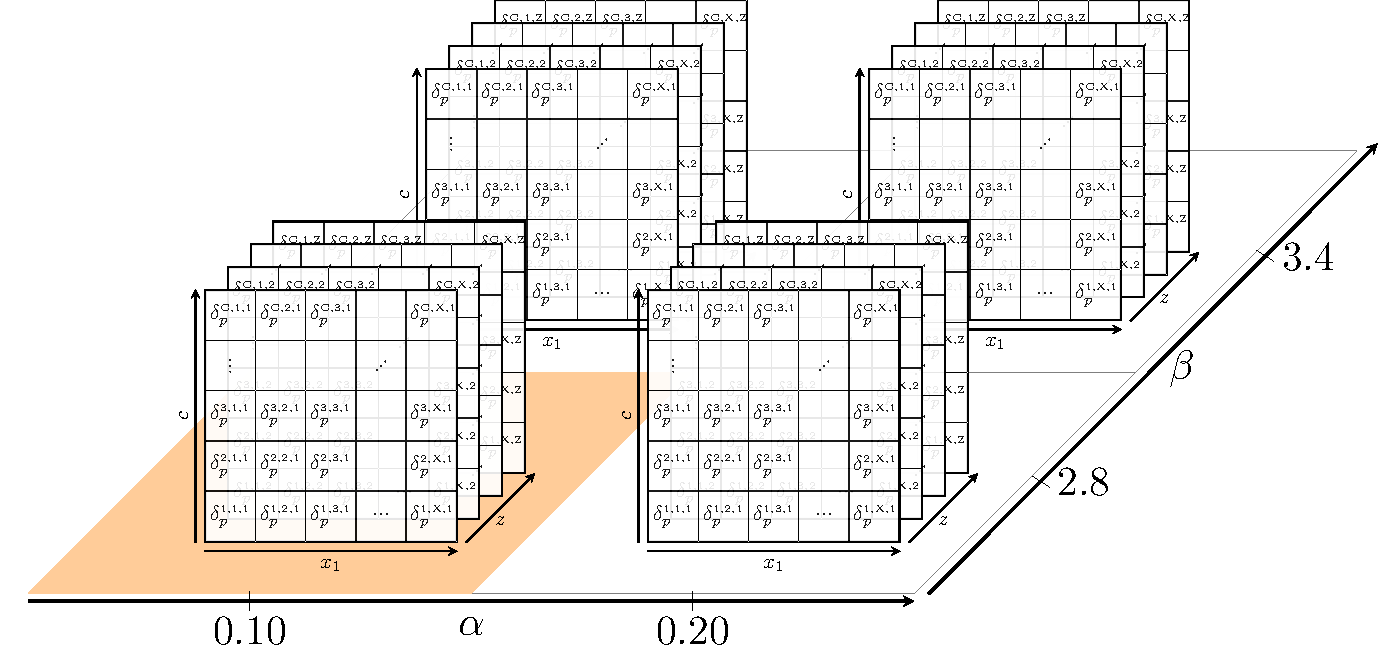
\includegraphics[width=2cm]{matrices_cube-selected.pdf}};
    \node[inter, below=of chainleft]
        (ab) {$\alpha$, $\beta$};
    \node[inner sep=0] (ableft) at ([shift={(-0.5cm,0)}]ab.west) {};
    % \begin{scope}[shift=(mcube)]
    %     \pgftransformcm{1}{0}{0.3}{0.5}{\pgfpoint{0cm}{0cm}}
    %     \draw[orange] (select) (-0.4,-0.3) circle (0.4cm) {};
    % \end{scope}
    \node[inter, below=of mcube]
    (dbias) {$\delta\mu_{\rm biais}(\rm 5D)$};
                %{$\delta\mu_{\rm biais} \triangleq -
                %(\delta_{m_B}+\alpha\delta_{x_1}-\beta\delta_c)$};
    \node[inter]
        (mu) at (data|-dbias) {$\mu$};
    \node[add, scale=2]
        (addbox) at ($(mu)!0.5!(dbias)$) {};
    \node[inter, below=of addbox]
        (mb) {$\mu \rightarrow \mu^*$};
    \node[circle, draw, fill=white, below=of mb]
        (chi2) {$\chi^2$};
    \node[draw, fill=white, scale=0.8, anchor=center]
        (label) at (chi2|-boxproc.south) {Meilleur ajustement};
    % \node[inter, below=of label, align=center]
    %     (bestfit) {$\mu^*, M_{z_i}$};
    % \node[add, scale=2]
    %     (add) at (data |- bestfit) {};
    \node[inout, below=of label]
        (res) {$\alpha$, $\beta$, $\gamma_{\rm env}$, $M_{z_i}$, $\sigma_{\mu}$};
    \node[process, below=of res]
        (wfit) {\texttt{wfit}};
    \node[inout, below=of wfit]
        (cosmo) {$w$, $\Omega_M$};
    % Plot lines
    \draw[->] (biascor) -- (chainrightop);
    \draw[->] (chainright) -- (mcube);
    \draw[->] (mcube) -- (dbias);
    % \draw[->] (dbias) |- (chi2.east);
    \draw[->, dashed] (chi2) -- (chi2 -| ableft) --
            node [diamond, draw, solid, rounded corners,
                  fill=Orchid!20, scale=0.5] {Minimisation}
            (ableft) -- (ab);
    \draw[->] (chi2) -- (label);
    \draw[->] (label) -- (res);
    \draw[->] (data) -- (chainleftop);
    \draw[->] (chainleft) --
            node[midway, fill=white, scale=0.5] {Essai}
        (ab);
    \draw[->] (ab) -- (mcube);
    \draw[->] (ab) -- (mu);
    \draw[->] (mu) -- (addbox);
    \draw[->] (dbias) -- (addbox);
    \draw[->] (addbox) -- (mb);
    % \draw[->] (bestfit) -- (add);
    % \draw[->] (add) -- (mb);
    \draw[->] (mb) -- (chi2);
    \draw[->] (res) -- (wfit);
    \draw[->] (wfit) -- (cosmo);
\end{tikzpicture}
\end{document}


